\justifying \setcounter{page}{39}\setcounter{chapter}{3}
\chapter{Campos de vectores}  
\begin{defi}
Sea $M$ una variedad diferenciable y $U \subset M$ abierto. Un \textbf{campo de vectores} $X$ sobre $U$ es una asignación a cada $p \in U$ de un elemento de $T_p M$. Escribiremos $X_p = v \in T_p M$.
\end{defi}
\begin{obs}
Con la noción introducida de fibrado tangente, podemos ver más rigurosamente la definición de un campo de vectores $X$ como una aplicación: $$\begin{tikzcd}
X:\hspace{-13mm} & U \rar & TM\\[-5mm]
& p \arrow[mapsto]{r} & X_p = (p,v) \in T_pM
\end{tikzcd}$$
\end{obs}
\begin{obs}
Si $U = M$, se dice que el campo es global, en otro caso se dice que es local.
\end{obs}

Si $X$ es un campo de vectores en $U \subset M$, para todo $p \in U$ existirá una carta $(V,\varphi \equiv (x_i))$ de $M$ con $p \in V$. Entonces, para todo $q \in U \cap V$, se tiene que $\left\{\dfrac{\partial}{\partial x_i}\Big|_q\right\}_{i=1}^n$ es una base de $T_q M$, con lo que 
$$X_q = \sum_{i=1}^n \lambda_i(q) \dfrac{\partial}{\partial x_i}\Big|_q \in T_q M$$
donde las $\lambda_i: U \cap V \to \mathbb{R}$ serán funciones, que denominaremos funciones coordenada de $X$ en $U \cap V$.

\begin{defi}
Sea $M$ una variedad diferenciable, $U \subset M$ un abierto y $X$ un \textbf{campo de vectores} en $U$. Se dice que $X$ es \textbf{diferenciable} si para todo $p \in U$ existe una carta $(V,\varphi)$ de $M$ con $p \in V$ de modo que las funciones coordenada de $X$ en la base $\left\{\dfrac{\partial}{\partial x_i}\Big|_q\right\}_{i=1}^n$ de $T_qM$, $q \in U \cap V$ son diferenciables. Al conjunto de los campos de vectores diferenciables en $U$ lo denotaremos por $\mathfrak{X}(U)$
\end{defi}
\begin{obs}
    Si las funciones coordenadas de $X$ son diferenciables para una carta $(V, \varphi)$ con $p\in V$, tambi\'en ser\'an diferenciables para cualquier carta que cubra a $p\in U$ en el dominio correspondiente.
\end{obs}

\begin{ejem}
Si $(U,\varphi\equiv(x_i))$ es una carta de $M$, entonces $\dfrac{\partial}{\partial x_i} \in \mathfrak{X}(U)$ para todo $i = 1,\dots,n$, siendo $\left(\dfrac{\partial}{\partial x_i}\right)_p = \dfrac{\partial}{\partial x_i}\Big|_p \in T_pM$.
\end{ejem}

\begin{prop}
Dado $U \subset M$ abierto, se verifica que $\mathfrak{X}(U)$ tiene estructura de $\mathcal{C}^{\infty}(U)$-módulo.

Fijado $U$, sabemos que $\mathcal{C}^{\infty}(U)$ es un anillo. Definiremos las operaciones de módulo como, para todos $X, Y \in \mathfrak{X}(U)$, $f \in \mathcal{C}^{\infty}(U)$ y $p \in U$:
$$(X+Y)_p = X_p + Y_p$$ $$(fX)_p = f(p) \cdot X_p$$
\end{prop}
\begin{dem}
\textcolor{red}{Ejercicio}
\end{dem}

\begin{defi}
Dado un abierto $U$, un campo de vectores $X$ en $U$ y una función $f: V \to \mathbb{R}$ de dominio abierto, se define la \textbf{aplicación del campo a la función} como la función
$$\begin{tikzcd}
X\,f:\hspace{-10mm} & U \cap V \rar & \mathbb{R}\\[-5mm]
& p \arrow[mapsto]{r} & X_p(f)
\end{tikzcd}$$
que es diferenciable.
\end{defi}

\begin{prop}
Sea $X$ un campo de vectores en un abierto $U \subset M$. Entonces $X$ es diferenciable si y solo si $\forall \, p \in U$ y $\forall \, f \in \mathcal{C}^{\infty}(p)$ se cumple que $Xf \in \mathcal{C}^{\infty}(p)$.
\end{prop}
\begin{dem} \, 

$\Rightarrow)$ Supongamos $X \in \mathfrak X(U)$, y sean $p \in U$ y $f \in \mathcal{C}^{\infty}(p)$, es decir, $f:V\to \mathbb{R}$ con $V\subset M$ abierto, $p \in V$ y $f$ diferenciable. Sea $(W,\varphi\equiv(x_i))$ una carta de $M$ con $p \in W$ y $W \subset U \cap V$. Entonces, para todo $q \in W$, $\displaystyle X_q = \sum_{i=1}^n \lambda_i(q) \dfrac{\partial}{\partial x_i}\big|_q$ donde cada $\lambda_i \in \mathcal C^{\infty}(W)$ por hip\'otesis. Por tanto, $$X_q(f) = \sum_{i=1}^n \lambda_i(q) \dfrac{\partial}{\partial x_i}\Big|_q (f)= \sum_{i=1}^n \lambda_i(q)  \dfrac{\partial (f\circ \varphi^{-1})}{\partial r_i}\Big|_{\varphi(q)} = \sum_{i=1}^n \lambda_i(q) \left( \dfrac{\partial (f\circ \varphi^{-1})}{\partial r_i} \circ \varphi\right) (q)$$ es diferenciable por ser composición de aplicaciones diferenciables. Luego $X\,f \in \mathcal{C}^{\infty}(W)$, y en particular, $X\,f \in \mathcal{C}^{\infty}(p)$, $\forall\, p\in U$.

$\Leftarrow)$ Veamos que si se cumple la condición establecida $X$ es diferenciable. Fijando $p \in U$, sea $(V,\varphi\equiv(x_i))$ carta de $M$ con $p \in V$. Entonces, para todo $q \in U \cap V$:$$X_q = \sum_{i=1}^n \lambda_i(q) \dfrac{\partial}{\partial x_i}\Big|_q\in T_qM$$donde $\lambda_i(q) = X_q(x_i)$. Como $x_i \in \mathcal{C}^{\infty}(V)$, en particular $x_i \in \mathcal{C}^{\infty}(q)$, con lo que por hipótesis $Xx_i \in \mathcal{C}^{\infty}(q)$ en $q \in U \cap V$, luego $Xx_i \in \mathcal{C}^{\infty}(U\cap V)$. \hfill $\blacksquare.$
\end{dem}

Se tiene, por tanto, si $X\in \mathfrak X(U)$, la correspondencia inducida por él entre los pseudoanillos de funciones diferenciables en un punto $p$:
$$\begin{tikzcd}
X:\hspace{-10mm} & \mathcal{C}^{\infty}(p) \rar & \mathcal{C}^{\infty}(p)\\[-5mm]
& f \arrow[mapsto]{r} & \tilde{X}(f) = X\,f
\end{tikzcd}$$

Igualmente, dado $v \in T_p M$ y $X \in \mathfrak{X}(U)$, si $U\subset M$ es abierto $\mathcal{C}^{\infty}(U)$ es un anillo y podemos calcular, para toda $f,g\in\mathcal{C}^{\infty}(U)$ y $\lambda \in \mathbb{R}$:
$$X(f+g) = X(f) + X(g)$$
$$X(\lambda\,f) = \lambda\,X\,f$$
$$X(f\cdot g) = (X\,f)\cdot g + f \cdot (X\,g)$$

\begin{defi}
Llamaremos \textbf{derivaciones} de $\mathcal{C}^{\infty}(U)$ a las aplicaciones $\mathcal{C}^{\infty}(U) \to \mathcal{C}^{\infty}(U)$ que verifiquen estas tres condiciones. Las denotaremos por $\mc Der(\mathcal{C}^{\infty}(U))$ y se demuestra que conforman un $\mathcal{C}^{\infty}(U)$-módulo.
\end{defi}

\begin{teo}
Sea $M$ una variedad diferenciable y $U \subset M$ un abierto. Entonces, $\mathfrak{X}(U)$ es isomorfo como $\mathcal{C}^{\infty}(U)$-módulo a $\mc Der(\mathcal{C}^{\infty}(U))$.
\end{teo}
\begin{dem}
Definamos la aplicación
$$\begin{tikzcd}
\mathfrak{X}(U) \arrow{r} & \mc Der(\mathcal{C}^{\infty}(U))\\[-4mm]
X \arrow[mapsto]{r} & \tilde{X}:\; \mathcal{C}^{\infty}(U) \arrow{r} & \mathcal{C}^{\infty}(U)\\[-7mm]
& f \arrow[mapsto]{r} & \tilde{X}\,f = X\,f
\end{tikzcd}$$
que está bien definida por los comentarios previos a este teorema. Veamos que es un morfismo de módulos: dada $g \in \mathcal{C}^{\infty}(U)$
$$\widetilde{X + fY}(g) = (X + fY)(g) = Xg + f\cdot Yg = \tilde{X}g + f\tilde{Y}g = (\tilde{X} + f\tilde{Y})(g)$$

Comprobemos ahora la inyectividad de esta aplicación: sea $X \in \mathfrak{X}(U)$ tal que $\tilde{X} = 0$, es decir, para toda $f \in \mathcal{C}^{\infty}(U)$, $\tilde{X}f = 0$. Veamos que $X = 0$, es decir, para todo $p \in U$, $X_p = 0$. Dado $p \in U$, sea $(V,\varphi\equiv (x_i))$ carta de $M$ con $p\in V$. Entonces, 
$$X_{q} = \mathlarger\sum_{i=1}^n X(x_i) \dfrac{\partial}{\partial x_i}\Big|_{q} \qquad \, \forall q \in U \cap V $$
en particular, si $p \in U\cap V$, $X_p =  \mathlarger\sum_{i=1}^n X_p(x_i) \dfrac{\partial}{\partial x_i}\Big|_p$. Sabemos que $x_i \in \mathcal{C}^{\infty}(V)$, usando una función meseta generamos $y_i \in \mathcal{C}^{\infty}(M)$ de modo que existe $W \subset V$ abierto con $p \in W$, donde $x_i|_W = y_i|_W$. Luego
$$X_p(x_i) = X_p(y_i) = X_p(y_i|_U) = \Big(\tilde{X}(y_i|_U)\Big)(p) = 0$$
y esto ocurre para todo $i = 1,\dots,n$, con lo que $X_p = 0$.

Por último, veamos la epiyectividad. Sea $D\in \mc Der(\mathcal{C}^{\infty}(U))$, queremos construir $X \in \mathfrak{X}(U)$ tal que $\tilde{X} = D$, es decir, para todo $p \in U$, tenemos que definir una derivación $X_p$ de $M$ en $p$. Dada $f \in \mathcal{C}^{\infty}(p)$, $f: V \subset M \to \mathbb{R}$ con $V$ abierto y $p \in V$. Usando una función meseta construimos $g \in \mathcal{C}^{\infty}(M)$ de modo que existe un abierto $W \subset V$ con $p \in W$, donde $f|_W = g|_W$. Definimos $$X_p(f) = \Big(D(g|_U)\Big)(p)$$
con lo que la definición no depende de la extensión utilizada, pues $D$ es derivación, por lo que dos extensiones de $f$ con las condiciones de dadas coinciden en un abierto que cotiene a $p$, y los $\big( D(g) \big)(p)$ de $D \in \mc Der(\mathcal C^{\infty}(U))$ dependen tan solo del valor local de $g$ (vale la misma demostración que la vista en $T_pM$). Se verifica fácilmente que:
\begin{itemize}
    \item $X_p(f_1 + f_2) = X_p(f_1) + X_p(f_2)$
    \item $X_p(\lambda f) = \lambda X_p(f)$
    \item $X_p(f_1 \cdot f_2) = X_p(f_1) \cdot f_2(p) + f_1(p) \cdot X_p(f_2)$
\end{itemize}
Con esto, tenemos definido $X$, que es un campo de vectores en $U$. Resta comprobar que es diferenciable, es decir, si $f \in \mathcal{C}^{\infty}(p)$ entonces $Xf \in \mathcal{C}^{\infty}(p)$. En efecto,
$$(Xf)(p) = X_p(f) = \Big(D(g|_U)\Big)(p)$$
que será diferenciable en un abierto que contenga a $p$, luego queda demostrado.
\end{dem}

\begin{obs}
En general, la composición de campos diferenciables no es un campo diferenciable.
\end{obs}

\begin{defi}
Sea $M$ variedad diferenciable, $U \subset M$ abierto y $X,Y \in \mathfrak{X}(U)$. Se llama \textbf{corchete o paréntesis de Lie}, denotado por $[X,Y]$ al campo de vectores en $U$ dado por: $\forall\;p\in U, f\in \mathcal{C}^{\infty}(p)$:
$$[X,Y]_p (f) = X_p(Yf) - Y_p(Xf)$$
\end{defi}
\begin{obs}
    Es claro que $[X,Y]$ es un campo de vectores en $U$, es decir, $\forall p \in U, \, [X,Y]_p \in T_pM$. 
\end{obs}

\begin{prop}
Si $X,Y \in \mathfrak{X}(U)$, entonces $[X,Y]\in \mathfrak{X}(U)$.
\end{prop}
\begin{dem}
A partir de la definición, podemos generar
$$\begin{tikzcd}
\left[X,Y\right]:\hspace{-10mm} & \mathcal{C}^{\infty}(U) \rar & \mathcal{C}^{\infty}(U)\\[-5mm]
& f \arrow[mapsto]{r} & X(Yf) - Y(Xf)
\end{tikzcd}$$
Veamos que este $[X,Y]$ es una derivación de $U$: dadas $f,g\in \mathcal{C}^{\infty}(U)$ se tiene que
\begin{itemize}
    \item $[X,Y](f+g) = X(Yf + Yg) - Y(Xf + Xg) = X(Yf) - Y(Xf) + X(Yg) - Y(Xg) = [X,Y](f) + [X,Y](g)$
    \item $[X,Y](\lambda\,f) = X(\lambda Yf) - Y(\lambda Xf) = \lambda[X,Y](f)$
    \item Regla de Leibniz \[\begin{split} [X,Y](f \cdot g) & =  X(Y(f\cdot g)) - Y(X(f\cdot g))= \\ & = X((Yf)\cdot g+f \cdot (Yg)) - Y((Xf) \cdot g + f(Xg))= \\ & = X(Yf) \cdot g + \cancel{(Yf)\cdot (Xg)} + \cancel{(Xf)\cdot(Yg)} + f(X(Yg)) - \\& - Y(Xf)\cdot g - \cancel{(Xf)(Yg)} - \cancel{(Yf)(Xg)} - f(Y(Xg))= \\ & = \Big( X(Yf) - Y(Xf) \Big) \cdot g + f \cdot \Big( X(Yg) - Y(Xg)\Big) = \\ & = \Big([X,Y](f)\Big) \cdot g + f \cdot \Big([X,Y](g)\Big) \end{split}\]
\end{itemize}
Como hemos visto, toda derivación de $U$ es (por isomorfía) un elemento de $\mathfrak{X}(U)$.
\end{dem}

\begin{prop} 
$\forall X,Y,Z \in \mathfrak X(U)$ con $U \subset M$ abierto y $f\in \mathcal C^{\infty}(U), \, \lambda\in \mathbb R$, el corchete de Lie verifica las siguientes propiedades: \vspace{-3mm}
\begin{enumerate}
    \item Antisimetría: $[X,Y] = -[Y,X]$
    \item $\mathbb{R}$-bilinealidad $[X,Y+\lambda Z] = [X,Y]+\lambda[Y,Z]$
    \item $[X,fY] = f[X,Y] + (Xf) Y$, y en consecuencia, si $g \in \mathcal C^{\infty}(U)$,  $[fX,gY] = fg[X,Y] + f\cdot X(g) Y - g\,(Yf) X$
    \item Identidad de Jacobi: $[[X,Y],Z] + [[Y,Z],X] + [[Z,X],Y] = 0$
\end{enumerate}
\end{prop}
\begin{dem} \, \vspace{-3mm}
\begin{enumerate}
    \item \textcolor{red}{Directa, ejercicio}
    \item \textcolor{red}{Directa, ejercicio}
    \item Sea $g \in \mathcal{C}^{\infty}(U)$. Entonces $[X,fY](g) = X((fY)(g)) - (fY)(Xg) = X(f\cdot (Yg)) - f \cdot Y(Xg) = (Xf)(Yg) + f\cdot X(Y g) - f\cdot Y(X g) = ((Xf) \cdot Y)(g) + f([X,Y](g)) = ((Xf)\cdot Y + f[X,Y])(g)$
    \item Dada $g \in \mathcal{C}^{\infty}(U)$, calculemos $[X,[Y,Z]](g) = [X,Y](Zg) - Z([X,Y]g) = X(Y(Zg)) - Y(X(Zg)) -Z(X(Yg)) + Z(Y(Xg))$.
    
    Análogamente, escribiendo los otros t\'erminos de Id de Jacobi:
    $$[[Y,Z],X](g) = Y(Z(Xg)) - Z(Y(Xg)) - X(Y(Zg)) +  X(Z(Yg))$$
    $$[[Z,X],Y](g) = Z(X(Yg)) - X(Z(Yg)) - Y(Z(Xg)) + Y(X(Zg))$$
    Se comprueba que la suma de las tres expresiones es $0$.
\end{enumerate}
Con estas propiedades se dice que $\mathfrak X(U)$ es un \'algebra de Lie.
\end{dem}


\begin{prop}
Sea $(U,\varphi\equiv (x_i))$ una carta de $M^n$. Entonces $$\left[\dfrac{\partial}{\partial x_i}, \dfrac{\partial}{\partial x_j}\right] = 0 \qquad \forall i,j = 1,\dots,n$$
\end{prop}
\begin{dem}
Sea $f \in \mathcal{C}^{\infty}(U)$. 
\[ \begin{split}
\left[\dfrac{\partial}{\partial x_i}, \dfrac{\partial}{\partial x_j}\right](f)&  =  \dfrac{\partial}{\partial x_i}\left(\dfrac{\partial}{\partial x_j}(f)\right) - \dfrac{\partial}{\partial x_j}\left(\dfrac{\partial}{\partial x_i}(f)\right) = \\ & = \dfrac{\partial}{\partial x_i}\left(\dfrac{\partial (f\circ \varphi^{-1})}{\partial r_j} \circ \varphi \right) - \dfrac{\partial}{\partial x_j}\left(\dfrac{\partial (f\circ \varphi^{-1})}{\partial r_i} \circ \varphi \right)  = \\ & = \dfrac{\partial}{\partial r_i} \left(\dfrac{\partial (f\circ \varphi^{-1})}{\partial r_j} \circ \varphi \circ \varphi^{-1} \right) \circ \varphi - \dfrac{\partial}{\partial r_j} \left(\dfrac{\partial (f\circ \varphi^{-1})}{\partial r_i} \circ \varphi \circ \varphi^{-1} \right) \circ \varphi= \\ & = \left(\dfrac{\partial (f\circ \varphi^{-1})}{\partial r_i \partial r_j} - \dfrac{\partial (f\circ \varphi^{-1})}{\partial r_j \partial r_i} \right) \circ \varphi = 0 \end{split}\]
Donde en el último paso hemos aplicado el lema de Schwartz en $\mathbb{R}^n$.
\end{dem}
\begin{ejem}
    Sean $\{x,y,z\}$ coordenadas de $\mathbb R^3$, consideremos los campos 
    $$X=xz\pd{}{x}+\pd{}{y}\qquad Y=\sin(z)\pd{}{x} + y^2 \pd{}{z} \quad X,Y \in \mathfrak X(\mathbb R^3)$$
    entonces
    \[ \begin{split}
        [X,Y]_X & = \left[xz\pd{}{x}+\pd{}{y}, \sin(z)\pd{}{x} + y^2 \pd{}{z} \right] = \\ & = \left[ xz\pd{}{x}, \sin(z)\pd{}{z}\right] + \left[ xz\pd{}{x}, y^2 \pd{}{z}\right]+\left[ \pd{}{y}, \sin(z) \pd{}{z} \right]+\left[ \pd{}{y},y^2 \pd{}{z} \right] = \\ & = \sin(z)\left[ xz\pd{}{x}, \pd{}{z}\right] + \left( xz \pd{}{x}\right) \cancelto{0}{\sin(z) \pd{}{x}} + y^2 \left[ xz\pd{}{x}, \pd{}{z} \right] +  \left( xz \pd{}{x}\right) \cancelto{0}{y^2 \pd{}{z}} + \\ & +
        \sin(z) \cancelto{0}{\left[ \pd{}{x},\pd{}{y}\right]} + \pd{}{y} (\sin(z)) \pd{}{x} + y^2 \cancelto{0}{\left[ \pd{}{y},\pd{}{z}\right]} + \pd{}{y} y^2 \pd{}{z} = \\ & = xz\sin(z)\left[ xz\pd{}{x}, \pd{}{z}\right] -\sin(z)\pd{}{x} (xz) \pd{}{x} + szy^2 \left[ \pd{}{x}, \pd{}{z}\right] - y^2 \pd{}{z} (xz) \pd{}{x} + 2y \pd{}{z} = \\ & = (-z\sin(z)-xy^2)\pd{}{x} + 2y \pd{}{z}
    \end{split}\]
\end{ejem}

Sea $f:M\to N$ diferenciable $X \in \mathfrak{X}(M)$. Para todo $p \in M$, $f_{*,p}(X_p) \in T_{f(p)}N$. En general, esto no produce un campo de vectores en $N$, tal vez $f(M)$ no es abierto en $N$, si $f$ no es inyectiva. Esto motiva la siguiente
\begin{defi}
Sea $f:M\to N$ una aplicación diferenciable, $X \in\mathfrak{X}(M)$ e $Y \in \mathfrak{X}(N)$. Se dice que $X$ e $Y$ están \textbf{$f$-relacionados}, denotándolo por $X \overset{f}{\sim} Y$, si para todo $p \in M$, $f_{*,p}(X_p) = Y_{f(p)} \forall \, p \in U$.
\end{defi}

\begin{lem}
En particular, si $g \in \mathcal{C}^{\infty}(f(p))$:
$$f_{*,p}(X_p))(g) = X_p(g \circ f) = (X(g \circ f))(p)$$
$$Y_{f(p)}(g) = (Yg)(f(p)) = ((Yg)\circ f)(p)$$
Por lo que los campos están $f$-relacionados si y solo si $X(g\circ f) = (Yg) \circ f$.
\end{lem}

\begin{prop}
Sean $X_1,X_2 \in \mathfrak{X}(M)$, $Y_1,Y_2 \in \mathfrak{X}(N)$, $f:M \to N$ diferenciable y $X_1 \overset{f}{\sim} Y_1, X_2 \overset{f}{\sim} Y_2$. Entonces, se verifica que $[X_1,X_2]\overset{f}{\sim} [Y_1,Y_2]$.
\end{prop}
\begin{dem} $X_1\sim Y_1$ $\forall p \in M$, es decir que $f_{*,p}(X_1)=(Y_1)_{f(p)} \in T_{f(p)}N$. As\'i pues, $\forall g \in \mathcal{C}^{\infty}(f(p))$ se verifica el anterior lema y se demuestra, tambi\'en para $X_2 \sim Y_2$. Entonces,
$$(f_{*,p}([X_1,X_2]_p(g)=[X_1,X_2]_p(g \circ f) = (X_1)_p(X_2(g \circ f)) - (X_2)_p(X_1(g \circ f)) = $$ $$=(X_1)_p((Y_2 g)\circ f) - (X_2)_p ((Y_1 g) \circ f) = (Y_1(Y_2 g) \circ f)(p) - (Y_2(Y_1 g)) \circ f) (p) = ([Y_1,Y_2]_{f(p)}(g)) \circ f$$ 
\end{dem}

\section{Curvas integrales y flujo de un campo}
\begin{defi}
Sea $M$ una variedad diferenciable, $X \in \mathfrak{X}(U)$ donde $U \subset M$ es un abierto y $p \in U$. Una curva diferenciable $\sigma: I \subset \mathbb{R} \to M$, donde $I$ es un intervalo abierto, se dice que es una \textbf{curva integral de $X$} si para todo $t \in I$, $\sigma'(t) = X_{\sigma(t)}$. Además, se dice que la curva integral pasa por $p \in U$ en $t_0 \in I$ si $\sigma(t_0) = p$.

Es habitual exigir que $0\in I$ y que $p = \sigma(0)$.
\end{defi}
\begin{obs}
    Consideramos dominios $I$ que sean conexos y abiertos, que son intervalos. 
\end{obs}

\begin{prop}
Sea $M$ una variedad diferenciable, $X \in \mathfrak{X}(U)$ con $U \subset M$ abierto, entonces $\forall p \in U$ existe $\sigma: I \subset \mathbb R \longrightarrow M$ una curva integral de $X$ , con $0\in I$, tal que $\sigma(0)=p$. Adem\'as, si $\gamma: J \subset \mathbb{R} \to M$ es otra curva integral de $X$ con $\sigma(0) = p = \gamma(0)$, entonces $\sigma|_{I \cap J} = \gamma|_{I \cap J}$.
\end{prop}
\begin{dem}
Dado $p \in U$, existirá una carta $(V,\varphi\equiv (x_i))$ de $M$ con $p \in V$. Entonces
$$X|_{U \cap V} = \sum_{i=1}^n X(x_i) \frac{\partial}{\partial x_i}$$
Buscamos $\sigma: I \subset \mathbb R \longrightarrow M$ cuya lectura en coordenadas ser\'a $\varphi \circ \sigma(t) = (x_1(t),\dots,x_n(t))$ determina $\sigma$ localmente, es determinar $x_1(t), \ldots, x_n(t)$. El vector tangente es
$$\sigma'(t) = \sum_{i=1}^n \sigma'(t) (x_i) \frac{\partial}{\partial x_i}\Big|_{\sigma(t)}$$
y $\sigma$ ser\'a curva integral de $X$, $X_{\sigma(t)} = \sigma'(t)$ lo que conduce a
$$(X(x_i))(\sigma(t)) =  X_{\sigma(t)}(x_i) = \dfrac{d(x_i\circ \sigma)}{dt} \Big|_t$$
que es un sistema de ecuaciones diferenciales de primer orden. Fijada la condici\'on inicial $\sigma(0)=p$ es decir $x_i(0) = x_i(p)$ con $i=1,\dots,n$ el teorema de existencia de soluciones para las ecuaciones diferenciales ordinarias asegura la existencia de tal soluci\'on.
\end{dem}

\begin{obs} Del enunciado concluimos que la $\sigma$ es \'unica excepto por el dominio de definici\'on. Si $\sigma: I\subset \mathbb{R} \to M$ y $\tau: J \subset \mathbb{R} \to M$ son dos curvas integrales de $X$ con $\sigma(0) = p = \tau(0)$, entonces está bien definida y es diferenciable pudiendo definir
$$\begin{tikzcd}
I \cup J \rar & M\\[-6mm]
t \arrow[mapsto]{r} & \begin{cases}
\sigma(t) \quad t\in I\\
\tau(t) \quad t \in J
\end{cases}
\end{tikzcd}$$
y seguirá siendo una curva integral de $X$, con la misma condición inicial y ahora con un dominio mayor.

En general, buscaremos la curva integral con mayor dominio de definición, que será la unión de los dominios de todas las curvas integrales $\sigma$ de $X$ con $\sigma(0) = p$, esto es $\displaystyle \bigcup \{Dom(\sigma) \, / \, \sigma \text{ curva integral de } X \, / \, \sigma(0)=p\}$. Llamaremos a esta\textbf{ curva integral maximal}.

En la demostraci\'on, $\sigma(I)\subset V$ abierto coordenado. La curva integral maximal, en general no tiene su imagen dentro de 1 abierto coordenado. 
\end{obs}
\begin{ejem}
    Sea $X=\pd{}{x} + xy \pd{}{y} \in \mathfrak X(\mathbb R^2)$. Buscamos $\sigma(t) = (x(t),y(t))$, de donde sacamos $\sigma'(t) = x'(t) \pd{}{x}\big|_{\sigma(t)} + y'(t) \pd{}{y}\big|_{\sigma(t)}$, y entonces
    $$X_{\sigma(t)} = \pd{}{x} \Big|_{\sigma(t)}+ x(t)y(t) \pd{}{y} \Big|_{\sigma(t)}$$
    de forma que $\sigma'(t)=X_{\sigma(t)}$, teniendo el sistema de ecuaciones diferenciales
    $$\begin{cases}
        x'(t)=1 \\ y'(t)=x(t)y(t)
    \end{cases}$$ 
para una condici\'on $\sigma(0)=(x_o,y_o) \in \mathbb R^2$ eliminando de la notaci\'on la dependendcia de la $t$,
$$\begin{cases}
        x'=1 \\ y'=xy \\ x(0)=x_o \\ y(0)=y_o
    \end{cases}$$ 
Resolviendo,
$$x(t)=t+x_o \quad y(t)=y_o e^{\nicefrac{1}{2} t^2+x_ot}$$
luego
$$\sigma(t) = \left(t+x_o , y_o \, e^{\nicefrac{1}{2} t^2+ x_o \, t}\right)$$
Podemos observar en las siguientes figuras el campo $X$ y la familia de curvas $\sigma(t)$, pudiendo observar c\'omo cada curva tiene por vector tangente a los del campo:
$$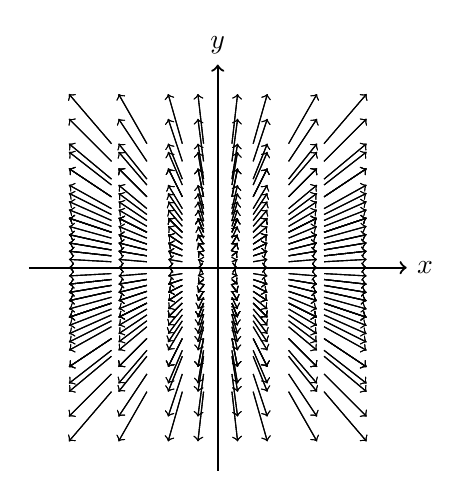
\begin{tikzpicture}[scale=0.6]
\draw[->, thick] (-4,0)--(4,0) node[right] {$x$};
\draw[->, thick] (0,-4.3)--(0,4.3) node[above] {$y$};

\def\factor{0.4}
\foreach \c in {-1.5,-1,-0.5,-0.2,0.2,0.5,1,1.5} {
\foreach \x in {-1.5,-1,-0.5,0.5,1,1.5} {
    \foreach \y [evaluate=\y as \r using int(ceil(abs(\x)+abs(\y)))] in {-1.75,-1.5,...,1.75}{
            \ifthenelse{\r=0}{}{\draw[->] (\c*1.5,\x*\y)--++(\factor*\c*1.5,\factor*\x*\y);}
    }
  }
}
\end{tikzpicture} \qquad 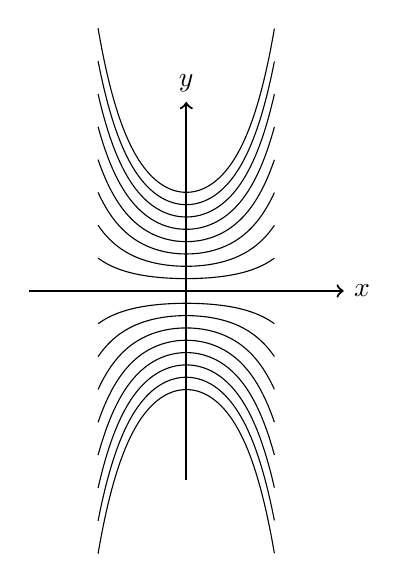
\begin{tikzpicture}[scale=0.8]
\draw[->, thick] (-2.5,0)--(2.5,0) node[right] {$x$};
\draw[->, thick] (0,-3)--(0,3) node[above] {$y$};

\foreach \xo in {-0.7,0.7} {
    \foreach \yo [evaluate=\yo as \r using int(ceil(abs(\xo)+abs(\yo)))] in {-2,-1.75,...,2}{
            \ifthenelse{\r=0}{}{\draw plot[domain=-0.7:0.7, samples=100] (\x + \xo, {\yo * exp(0.5 * \x * \x + \xo * \x)});}
    }
}
\end{tikzpicture}$$
            
Adem\'as, el dominio es todo $\mathbb R$, pues no hay puntos peculiares, $\sigma: \mathbb R \longrightarrow \mathbb R$.
\end{ejem}
\begin{ejem}
    Sea $M=(0, +\infty) \subset \mathbb R$, sea el campo $Y=\frac{1}{x} \frac{\partial}{\partial x} \in \mathfrak X(M)$, buscamos $\sigma(t)=x(t)$, $x'(t) = \frac{1}{x(t)}$, teni\'endose el sistema
    $$\begin{cases}
        x' = \frac{1}{x} \\ x(0)=x_o
    \end{cases} \Rightarrow \sigma(t) = \sqrt{2y+x_o^2}$$
    luego $\sigma: I = (-\nicefrac{1}{2} \, x_o^2, +\infty) \longrightarrow M$ es decir, el dominio de definici\'on, en general, depende de las condiciones iniciales. 
\end{ejem}

\begin{defi}
Se dice que un \textbf{campo de vectores} es \textbf{completo} si la curva integral maximal que pasa por $p$ en $t=0$ está definida para toda $t \in \mathbb{R}$.
\end{defi}
\begin{ejem}
    El que vimos en $\mathbb R^2$ es completo y el que vimos en $M=(0,\infty)$ no es completo.
\end{ejem}

\begin{prop}
Sea $M$ una variedad diferenciable y $X \in \mathfrak{X}(M)$, $p \in M$. Si $\sigma_p:(a,b)\subset \mathbb{R}\to M$ es la curva integral maximal de $X$ que en $t=0$ pasa por $p \in M$. Para todo $t_o \in [a,b]$, $q=\sigma_p(t_o)$ entonces la curva $\sigma_q(t) = \sigma_p(t + t_0)$ definida por $\sigma_q:(a-t_0,b-t_0) \to M$, es la curva integral maximal de $X$ que en $t=0$ pasa por $q = \sigma_p(t_o) \in M$.
\end{prop}
\begin{dem}
\textcolor{red}{Ejercicio}
\end{dem}

\begin{obs}
Si $(a,b)$ no estuviese acotado superior o inferiormente, tampoco lo estaría $(a-t_0,b-t_0)$.
\end{obs}

\begin{teo}
Sea $M$ una variedad diferenciable y $X \in \mathfrak{X}(M)$. Para todo $p \in M$, existe un intervalo abierto $I_p \subset \mathbb{R}$ con $0 \in I_p$, un abierto $U_p \subset M$ con $p \in U_p$ y una aplicación diferenciable $\Psi_p:I_p \times U_p \to M$ tal que:
\begin{enumerate}[a)]
    \item Para todo $q \in U_p$, la aplicaci\'on $\sigma_q(t) = \Psi_p(t,q)$ definida en $I_p$ es curva integral de $X$ con $\sigma_q(0)=q$. En particular, $\Psi_p(0,q) = q$ para todo $q \in U_p$.
    \item Si $J_p \subset \mathbb R$ y $V_p \subset M$ son abiertos y existe otra aplicación diferenciable $\Phi_p:J_p \times V_p \to M$ que cumpla las condiciones de a), entonces $$\Psi_p(t,q) = \Phi_p(t,q) \quad \forall\; (t,q) \in (I_p\cap J_p) \times (U_p \cap V_p)$$
\end{enumerate}
\end{teo}
\begin{dem}
Ver \textbf{Currás}, se demuestra aplicando la dependencia diferenciable de las soluciones de SEDO respecto a las condiciones iniciales \textcolor{red}{(gracias Ricardo por tanto)}.
\end{dem}
\begin{obs}
Los dominios de cada $\Psi_p$, $I_p \times U_p$ no quedan completamente determinados por $X$ ni $p\in M$. 
\end{obs}
\begin{obs}
Si el campo $X$ es completo, podemos tomar los $I_p = \mathbb{R} \, \forall p \in M$.
\end{obs}

\begin{defi}
A la familia $\{\Psi_p\}_{p \in M}$ de aplicaciones definidas en el teorema anterior se le llama \textbf{flujo de $X$} .
\end{defi}

\begin{teo}
Sea $M$ una variedad diferenciable y $X \in \mathfrak{X}(M)$. Para todo $t \in \mathbb{R}$, se define $D_t = \{p \in M \;/\; t$ pertenece al dominio de definición de la curva integral maximal de $X$ con condición inicial en $p\} \subset M$. Entonces:
\begin{enumerate}[a)]
    \item Para todo $t \in \mathbb{R}$, $D_t$ es abierto y $\underset{t > 0}{\bigcup} D_t = M = \underset{t < 0}{\bigcup} D_t$
    \item Si $\tau_t:D_t \subset M \to M$ es la aplicación definida por $\tau_t(p) = \sigma_p(t)$, donde $\sigma_p$ es la curva integral maximal de $X$ con condición inicial $p$, entonces $\tau_t$ es diferenciable.
    \item Para todo $t\in \mathbb{R}$, $\tau_t(D_t) = D_{-t}$
    \item $\tau_o : D_o = M \to M$ es la identidad: $\tau_o(p) = \sigma_p(0) = p$, $\tau_o=Id$.
    \item Para todos $t,s \in \mathbb{R}$, el dominio $Dom(\tau_t\circ \tau_s
    ) \subset Dom(\tau_{t+s})$ y son iguales cuando $t,s$ tienen el mismo signo. En el menor dominio se cumple que $\tau_t \circ \tau_s = \tau_{t+s}$
    \item Para todo $t \in \mathbb{R}$, $\tau_t$ es un difeomorfismo con inversa $(\tau_t)^{-1} = \tau_{-t}$.
\end{enumerate}
\end{teo}

\begin{obs} \,
\begin{itemize}
\item Si $X$ es completo, entonces $D_t = M$ para todo $t$. En tal caso, las aplicaciones $\tau_t:M\to M$ podrán componerse en todo caso, y a la familia $\{\tau_t\}_{t\in \mathbb{R}}$ se le llama \textbf{grupo uniparamétrico de transformaciones}. En efecto, la composición es una ley de grupo por las propiedades anteriores.
\item Si $X$ no es completo, algún $D_t$ depende del $t$ y en algún caso $Dom(\tau_t\circ \tau_s) \subsetneqq Dom(\tau_{t+s})$. A la familia $\{\tau_t\}_{t\in \mathbb{R}}$ se le llama \textbf{grupo uniparamétrico local de transformaciones}.
\item Si tenemos una familia de aplicaciones diferenciables $\tau_t:U_t \subset M \to M$ que verifican las propiedades a), d), e) (y en consecuencia f) ) del teorema anterior, se llama \textbf{generador infinitesimal} de la familia $\{\tau_t\}_{t \in \mathbb{R}}$ al campo de vectores
$$X_p = \sigma'_p(0) \qquad \text{donde } \sigma_p(t) = \tau_t(p) \;\forall\; p\in M, t\in \mathbb{R}$$
Se demuestra que $\sigma$ y $X$ son diferenciables, y que el grupo uniparamétrico generado por este campo es precisamente $\{\tau_t\}_{t \in \mathbb{R}}$.
\end{itemize}
\end{obs}
\begin{ejem}
    Sea $M=(a,\infty)\subset \mathbb R$ y el campo $X=\frac{1}{x} \frac{\partial}{\partial x}$, la curva integral maximla de $X$ que pasa por $x \in M$ estaba definida por
    $$\bt \sigma_x : (-\frac{1}{2}x^2, \infty) \arrow{r} & M \\[-5mm] t \arrow[mapsto]{r} & \sqrt{2t+x^2} \et$$
    Como dominio del flujo $\Psi_x$ podemos tomar $I_x=\left(-\frac{1}{4}x^2,\infty\right), \, U_x=\left(\frac{\sqrt{2}}{2}x,\infty\right)$ de modo que construimos el flujo
    $$\bt \Psi_x : I_x \times U_x \arrow{r} & M \\[-5mm] (t,y) \arrow[mapsto]{r} & \sqrt{2t+y^2} \et$$
    de forma que 
    $$D_t = \begin{cases}
        M & t \geq 0 \\ (\sqrt{-2t},+\infty) & t < 0
    \end{cases}$$
    y por tanto 
    $$\bt \tau_t : D_t \arrow{r} & M \\[-5mm] x \arrow[mapsto]{r} & \sqrt{2t+x^2} \et$$
    y queda comprobar que para $s=-1, t=2$ resulta que $Dom (\tau_t\circ \tau_s)=(\sqrt{2}, \infty) \subsetneqq M = Dom(\tau_{t+s})$ y comprobar la ley de grupo. 
\end{ejem}



